
\section{Tree-structured neural networks} \label{methods}

We limit the scope of our experiments in this paper to neural network models 
that adhere to the linguistic \ii{principle of
 compositionality}, which says that the meanings for complex
expressions are derived from the meanings of their parts
via specific composition functions \cite{Partee84,Janssen97}. In our
distributed setting, word meanings are embedding vectors of dimension $N$. A learned
composition function maps pairs of them to single phrase vectors of dimension $N$, 
which can then be merged again to represent more complex
phrases, forming a tree structure. Once the entire sentence-level representation has been
derived at the top of the tree, it serves as a fixed-dimensional input for some subsequent layer function.

\begin{figure}[tp]
  \centering
  \begin{subfigure}[t]{0.45\textwidth}
\centering
\scalebox{0.75}{
 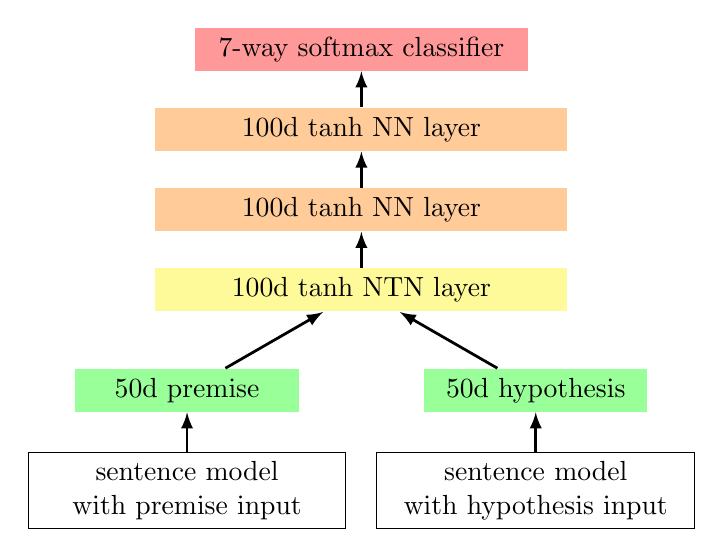
\begin{tikzpicture}
    \def\dx{21pt}
    \def\dy{29pt}

    \tikzstyle{label}=[text width=40mm,align=center]    
    \tikzstyle{softmax}=[fill=red!40,text width=40mm,align=center]
    \tikzstyle{preclass}=[fill=orange!40,text width=50mm,align=center]
    \tikzstyle{e}=[fill=green!40,text width=26mm,align=center]
    \tikzstyle{m}=[draw=black,text width=38mm,align=center]    
    
    \node[softmax]  (softmax) at (0*\dx,6*\dy) {7-way softmax classifier};
    \node[preclass]  (pc3) at (0*\dx,5*\dy) {100d $\tanh$ NN layer};
    \node[preclass]  (pc2) at (0*\dx,4*\dy) {100d $\tanh$ NN layer};
    \node[preclass,fill=yellow!40]  (pc1) at (0*\dx,3*\dy) {100d $\tanh$ NTN layer};
    \node[e]  (pe) at (-3*\dx,1.75*\dy) {50d premise};
    \node[e]  (he) at (3*\dx,1.75*\dy) {50d hypothesis};
    \node[m]  (pem) at (-3*\dx,0.5*\dy) {sentence model\\ with premise input};
    \node[m]  (hem) at (3*\dx,0.5*\dy) {sentence model\\ with hypothesis input};    
    
    \pgfsetarrowsend{latex}
    \tikzstyle{fwd} = [draw=black, line width=1pt]

          \draw [fwd] (pc3) -- (softmax);
          \draw [fwd] (pc2) -- (pc3);
          \draw [fwd] (pc1) -- (pc2);
          \draw [fwd] (pe) -- (pc1);
          \draw [fwd] (he) -- (pc1);
          \draw [fwd] (hem) -- (he);
          \draw [fwd] (pem) -- (pe);

  \end{tikzpicture}}
  
 \caption{The general architecture shared across models.}\label{fig:model:top}
  
\end{subfigure}

\begin{subfigure}[t]{0.45\textwidth}
  \centering
\scalebox{0.75}{
 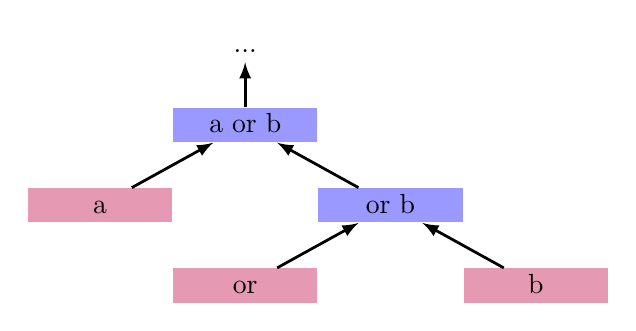
\begin{tikzpicture}
    \def\dx{21pt}
    \def\dy{29pt}


    \tikzstyle{word}=[fill=purple!40,text width=16mm,text height=2mm,align=center]
    \tikzstyle{node}=[fill=blue!40,text width=16mm,text height=2mm,align=center]
    \tikzstyle{empty}=[fill=blue!0,text width=8mm,text height=2mm,align=center]

    \node[empty]  (null) at (0*\dx,7*\dy) {...};
    \node[node]  (aorb) at (0*\dx,6*\dy) {a or b};
    \node[word]  (a) at (-2.5*\dx,5*\dy) {a};
    \node[node]  (orb) at (2.5*\dx,5*\dy) {or b};
    \node[word]  (or) at (0*\dx,4*\dy) {or};
    \node[word]  (b) at (5*\dx,4*\dy) {b};
    
    
    \pgfsetarrowsend{latex}
    \tikzstyle{fwd} = [draw=black, line width=1pt]

          \draw [fwd] (or) -- (orb);
          \draw [fwd] (b) -- (orb);
          \draw [fwd] (a) -- (aorb);
          \draw [fwd] (orb) -- (aorb);
          \draw [fwd] (aorb) -- (null);
  \end{tikzpicture}}
  
     \caption{The architecture for the TreeRNN and TreeRNTN sentence models. Terminal nodes are learned embeddings and nonterminal nodes are either NN or NTN layers with $\tanh$ nonlinearities.}\label{fig:model:tree}
  
  \end{subfigure}
 \vspace{0.5cm}
  
\begin{subfigure}[t]{0.45\textwidth}
  \centering
\scalebox{0.75}{
 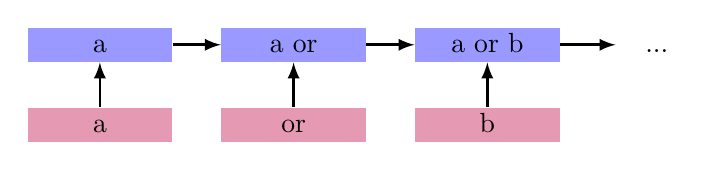
\begin{tikzpicture}
    \def\dx{35pt}
    \def\dy{29pt}


    \tikzstyle{word}=[fill=purple!40,text width=16mm,text height=2mm,align=center]
    \tikzstyle{node}=[fill=blue!40,text width=16mm,text height=2mm,align=center]
    \tikzstyle{empty}=[fill=blue!0,text width=8mm,text height=2mm,align=center]

    \node[word]  (a) at (-3*\dx,1*\dy) {a};
    \node[node]  (aN) at (-3*\dx,2*\dy) {a};
    
    \node[word]  (or) at (-1*\dx,1*\dy) {or};
    \node[node]  (orN) at (-1*\dx,2*\dy) {a or};
    
    \node[word]  (b) at (1*\dx,1*\dy) {b};
    \node[node]  (bN) at (1*\dx,2*\dy) {a or b}; 
    
    \node[empty]  (nullN) at (2.75*\dx,2*\dy) {...}; 
    
    \pgfsetarrowsend{latex}
    \tikzstyle{fwd} = [draw=black, line width=1pt]

          \draw [fwd] (or) -- (orN);
          \draw [fwd] (b) -- (bN);
          \draw [fwd] (a) -- (aN);
          \draw [fwd] (aN) -- (orN);
          \draw [fwd] (orN) -- (bN);
          \draw [fwd] (bN) -- (nullN);
          
  \end{tikzpicture}}
  
   \caption{The architecture for the LSTM sentence model. Nodes in the lower row are learned embeddings and nodes on the upper row are LSTM units.}\label{fig:model:seq}
  
    \end{subfigure}
  \caption{In our model, two separate tree-structured networks build up vector representations for each of two sentences using either NN or NTN layer functions. A comparison layer then uses the resulting vectors to produce features for a classifier.} 
  \label{sample-figure}
\end{figure}

To apply these recursive models to our task, we propose the tree 
pair model architecture depicted in Fig.~\ref{sample-figure}. 
In it, the two phrases being compared are processed separately using a pair 
of tree-structured networks that share a single set of parameters. 
The resulting vectors are fed into a separate comparison
layer that is meant to generate a feature vector capturing the
relation between the two phrases. The output of this layer is then
given to a softmax classifier, which produces a
distribution over the seven relations represented in Table~\ref{b-table}.

For the sentence embedding portions of the network, we evaluate both TreeRNN models with
 the standard NN layer function \eqref{TreeRNN} and those with the more powerful neural tensor 
 network layer function
\eqref{TreeRNTN} proposed in \newcite{chen2013learning}. The nonlinearity $f(x) = \tanh(x)$ is applied
 elementwise to the output of either layer function.
%
\begin{gather} 
\label{TreeRNN}
\vec{y}_{\textit{TreeRNN}} = f(\mathbf{M} \colvec{2}{\vec{x}^{(l)}}{\vec{x}^{(r)}} + \vec{b}\,) \\
\label{TreeRNTN} 
\vec{y}_{\textit{TreeRNTN}} = \vec{y}_{\textit{TreeRNN}} + f(\vec{x}^{(l)T} \mathbf{T}^{[1 \ldots n]} \vec{x}^{(r)})
\end{gather} 
%
Here, $\vec{x}^{(l)}$ and $\vec{x}^{(r)}$ are the column vector
representations for the left and right children of the node, and
$\vec{y}$ is the node's output.  The TreeRNN concatenates them, multiplies
them by an $N \times 2N$ matrix of learned weights, and adds a bias $\vec{b}$. 
The TreeRNTN adds a learned full rank third-order tensor 
$\mathbf{T}$, of dimension $N \times N \times N$, modeling
multiplicative interactions between the child vectors. 
The comparison layer uses the same layer function as the
composition layers (either an NN layer or an NTN layer) with
independently learned parameters and a separate nonlinearity function.
Rather than use a $\tanh$ nonlinearity here, we found better results with the leaky rectified linear function
\cite{maasrectifier}: $f(x)=\max(x, 0) +
0.01\min(x, 0)$. 

Other strong tree-structured models have been proposed in past work
\cite{sochergrounded,irsoydeep,tai2015improved}, but
we believe that these two provide a valuable case study, and that positive results on 
here are likely to generalize well to stronger models.

To run the model forward, we assemble the two tree-structured networks so as to match the structures provided for each phrase, which are either included in the source data or given by a parser.
The word vectors are then looked up from the vocabulary embedding matrix $V$ (one of the learned model parameters), and
the composition and comparison functions are used to pass information
up the tree and into the classifier. For an objective
function, we use the negative log likelihood of the
correct label with tuned L2 regularization.

We initialize parameters uniformly, using the range $(-0.05, 0.05)$ for layer parameters
and $(-0.01, 0.01)$ for embeddings, and train the model using stochastic gradient descent (SGD)
with learning rates computed using AdaDelta \cite{zeiler2012adadelta}.
The classifier feature vector is fixed at 75 dimensions and 
the dimensions of the recursive layers are tuned manually.
Training times on CPUs vary from hours to days across experiments.
On the experiments which use artificial data, we report mean
results over five fold cross-validation, where
variance across runs is typically no
more than two percentage points. In addition, because the classes are not necessarily balanced, 
we report both accuracy and macroaveraged F1.\footnote{We compute macroaveraged F1 
as the harmonic mean of average precision and average recall, both computed
for all classes for which there is test data, setting precision to 0 
where it is not defined.}
Source code and generated data can be downloaded from \url{http://stanford.edu/~sbowman/}.

